\documentclass{article}
\usepackage{graphicx}
\usepackage{float}
\usepackage{mathtools}
\usepackage[acronym]{glossaries}

\author{}
\title{ELEC 302-81\\ Lab 5\\ Motor Torque, Speed, Losses, and Efficiency}
\date{\today}

\loadglsentries{acronyms}
\makeglossaries
\begin{document}

\maketitle

\begin{center}
  \begin{tabular}{lr}
    Date Performed: & February 25, 2013 \\
    Partners: & Rawley Dent \\
              & Charles Pittman \\
    Instructor: & Dr. Weatherford
  \end{tabular}
\end{center}

\pagebreak

%\setlength\parindent{0pt}

\section{Purpose of Experiment}

In this experiment, the \gls{pm} and \gls{dyno} modules were used to measure
torque, speed, power, and efficiency of a DC motor. This experiment consisted
of three parts. Part 1 involved only the \gls{pm} module, and the basic
operation of the \gls{pm} was studied and the friction torque generated without
a load was measured. Part 2 involved the \gls{dyno} acting as a load to the
\gls{pm}, and the changes in torque due to the addition of the \gls{dyno} were
studied. Part 3 involved an experimental study of the \gls{pm} power losses and
efficiency.

\section{Procedure}

\subsection{EMS Workstation Set-up}

The main power switch and voltage control knob were verified to be OFF and
turned fully CCW, respectively. The voltmeter selector switch was set to
position 7--N. The Low Power Inputs for the \gls{pm}/\gls{dyno} module and the
\gls{dai} were connected to the 24-V supply, which was then turned on. The
\gls{dai} USB was connected to the computer. On the computer, the file for Lab
05 was opened in the EMS application, and the metering window was set to
continuous refresh.

\subsection{Prime Mover Operation}

\label{part1} The circuit represented by Figure~\ref{fig:circuit_01} was
constructed. Special, low-power connection wires were used to connect the
torque ($T$), speed ($N$), and ground terminals from the \gls{pm}/\gls{dyno}
modules to the \gls{dai} module. On the \gls{pm}/\gls{dyno} control switches,
the mode switch was set to \gls{pm} and the display switch was set to Speed
($n$). The main voltage supply was turned ON and the DC supply voltage was
adjusted to 30-V. Both the installed analog EMS voltmeter and the metering
window were monitored for proper indications. The DC voltage ($E_1$), the speed
($n$), indicated on the \gls{pm} digital display, and the speed ($N$) and
direction of rotation were measured and recorded in Table~\ref{tab:table_01}.
On the \gls{pm}/\gls{dyno} module, the Display switch was set to the Torque
position. The friction torque ($T_f$), indicated on the \gls{pm} digital
display and the torque ($T$), indicated in the metering window were measured
and recorded in Table~\ref{tab:table_01}.  On the \gls{pm}/\gls{dyno} module,
the Mode switch was set to the {Dyn}. position.  After a few seconds, the Mode
was set back to the PM position. The main power switch was set to OFF the
voltage control knob was turned fully {CCW}. The polarity of the leads at the
\gls{pm} input was then reversed. The main power switch was turned ON and the
voltage supply was adjusted to 30-V. The DC voltage ($E_1$), the speed ($n$),
indicated on the \gls{pm} digital display, and the speed ($N$) and direction of
rotation of the \gls{pm} were recorded in Table~\ref{tab:table_01}. The main
power switch to was set to {OFF} and voltage control knob was was fully {CCW}.
The leads were then connected to their original polarity.

The power supply was set to {ON}. On the computer application, the Data Table
Applications window was opened. The \gls{pm} Voltage ($E_1$), speed ($N$), and
torque, ($T$), were checked as the values to be recorded in the table. Using
the voltage control knob, the \gls{pm} speed was increased in approximately
300-rpm increments from 0--2100-rpm. At each 300-rpm increment, the values for
$E_1$, $N$, and $T$ were recorded into the Data Table. This data is shown in
Table~\ref{tab:table_02}. The voltage control knob was set fully CCW, and the
main power switch set to {OFF}. On the computer application, the Graph window
was opened. The Graph window was set to obtain a plot of \gls{pm} Speed ($N$),
vs. \gls{pm} Voltage ($E_1$). The graph was created and then saved.  This graph
is shown in Figure~\ref{fig:plot_01}. The graph window was then set to obtain a
plot of \gls{pm} friction torque ($T$), vs. \gls{pm} Speed (rpm), shown in
Figure~\ref{fig:plot_02}.

\subsection{Dynamometer Operation}

\label{part2} A timing belt was used to couple the two modules of the
\gls{pm}/\gls{dyno} together. The module on the left acted as the \gls{pm}, and
the module on the right acted as the \gls{dyno}. The circuit represented by
Figure~\ref{fig:circuit_02} was constructed. The smaller sized leads were
connected to the T and N meters on the \gls{dyno} side. The 24-V supply was
connected to the \gls{pm}/\gls{dyno} and the \gls{dai} modules. On the \gls{pm}
module, the Mode switch was set to \gls{pm}, and the Display switch was set to
Speed. On the \gls{dyno} module, the Mode switch was set to DYN, the Display
switch was set to Torque, the Load Control Mode switch was set to Man., and the
Load Control knob was set to Min. (fully CCW). The main power switch was set ON
and the voltage control knob was adjusted until the \gls{pm} rotated at a speed
of 1500-rpm. On the \gls{pm} module, the Display switch was set to Torque.  The
opposition torque was then measured and recorded. This data is shown in
Table~\ref{tab:table_03}. The Display switch was returned to Speed. On the
\gls{dyno} module, the Load Control knob was slowly adjusted clockwise until
the torque on the digital display indicated 2.0 Nm. The voltage control knob
was then adjusted so that the \gls{pm} rotated at 1500-rpm. The opposition
torque ($T_{PM}$), indicated by the \gls{pm} digital display and the
non-corrected output torque ($T_{NC}$), in the metering window were measured
and recorded. These values are shown in Table~\ref{tab:table_03}. On the
computer in the metering window, the torque correction function (mode C) for
the torque meter was selected. The meter was then set to read the \gls{pm}
output torque corrected for belt friction and windage. The voltage control knob
was then adjusted so that the \gls{pm} rotated at 1500-rpm.  The corrected
torque ($T_C$) was then indicated in the metering window. This value was
recorded in Table~\ref{tab:table_03}. The voltage supply was set fully CCW and
the main power switch to OFF.

\subsection{Motor Losses and Efficiency}

\label{part3} The circuit represented by Figure~\ref{fig:circuit_02} was kept
connected on the EMS workstation.  On the \gls{pm} module, the Mode switch was
set to Prime Mover, and the Display switch was set to Speed. On the \gls{dyno}
module, the Mode switch was set to Dyn., the Display switch was set to Torque,
the Load Control Mode switch was set to Man., and the Load Control knob was
turned fully {CCW}. On the metering window, the torque correction function
(mode C) for the torque meter was selected. The voltage supply knob was then
adjusted so that the \gls{pm} rotated at 1500-rpm. On the \gls{dyno} module,
the Load Control knob was adjusted until the digital display indicated 1.0-Nm.
The \gls{dyno} speed ($N$), and the corrected output torque ($T_C$), from the
metering window were measured and recorded. These values are shown in
Table~\ref{tab:table_04}. The \gls{pm} mechanical output power ($P_{mech}$),
indicated on meter, $P_m$, the \gls{pm} electrical input power ($P_{in}$),
indicated on meter $PQS_1$, and the \gls{pm} efficiency ($\eta$), indicated on
meter $A$ were measured and recorded. These values are shown in
Table~\ref{tab:table_05}.

On the \gls{dyno} module, the Load Control knob was slowly adjusted CCW until
the indicated torque display read 0-Nm. The voltage control knob was then
adjusted until the \gls{pm} rotated at 1500-rpm. The Data Table Application was
opened on the computer. The \gls{pm} voltage ($E_1$), current ($I_1$),
electrical input power ($PQS_1$), speed ($N$), output torque ($T$), mechanical
output power ($P_{m}$), and efficiency ($A$), were set to be recorded in the
Data Table. On the \gls{dyno} module, the Load Control knob was adjusted so
that the torque indicated on its digital display increased from 0--2.0-Nm in
0.2-Nm increments.  For each increment value, the values to be recorded were
entered into the Data Table. These values are shown in
Table~\ref{tab:table_06}. The voltage control knob was set fully CCW and the
main power switch to {OFF}. The Graph window on the computer was then opened.
It was set to obtain a plot of \gls{pm} efficiency vs. \gls{pm} mechanical
output power. This graph was created and saved. It is shown in
Figure~\ref{fig:plot_03}. The 24-V power supply was then turned OFF and the
timing belt removed.

\section{Results}

\subsection{Prime Mover Operation}

\begin{table}[H]
  \centering
  \begin{tabular}{*{6}{c}}
    \textbf{Voltage} & \multicolumn{2}{c}{\textbf{Speed}} & \textbf{Direction}
    & \textbf{Friction} & \textbf{Torque} \\
    $E_1$ V & $n$ rpm & $N$ rpm & CW/CCW & $T_f$ Nm & $T$ Nm \\
    \hline
     30.10 &  503.0 &  509.6 &  CW & -0.18 & -1.60 \\
    -30.19 & -508.0 & -513.0 & CCW &   --- &   --- \\
  \end{tabular}
  \caption{\gls{pm} friction torque; \gls{pm} polarity reversal}
  \label{tab:table_01}
\end{table}

\begin{table}[H]
  \centering
  \begin{tabular}{*{3}{c}}
    \textbf{Voltage} & \textbf{Torque} & \textbf{Speed} \\
    $E_1$ V          & $T$ N-m         & $n$ rpm \\

    \hline

      0.04 &     0 &    0.43 \\
     18.84 & -0.15 &  308.54 \\
     35.60 & -0.17 &  607.85 \\
     53.00 & -0.18 &  913.84 \\
     70.23 & -0.19 & 1220.52 \\
     86.02 & -0.20 & 1502.90 \\
    102.99 & -0.21 & 1807.37 \\
    119.92 & -0.22 & 2107.53 \\
  \end{tabular}
  \caption{Recorded data when the \gls{pm} speed was increased}
  \label{tab:table_02}
\end{table}

\begin{figure}[H]
  \centering
  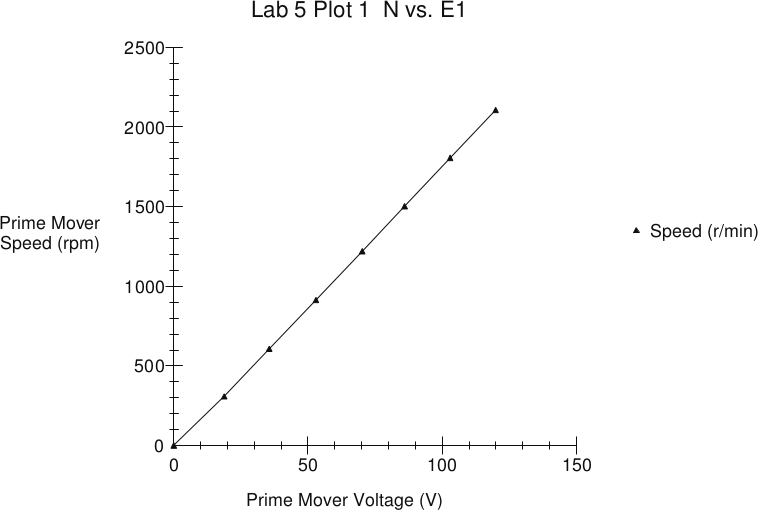
\includegraphics[width=\textwidth]{img/plot1}
  \caption{\gls{pm} Speed vs. \gls{pm} Voltage}
  \label{fig:plot_01}
\end{figure}

\begin{figure}[H]
  \centering
  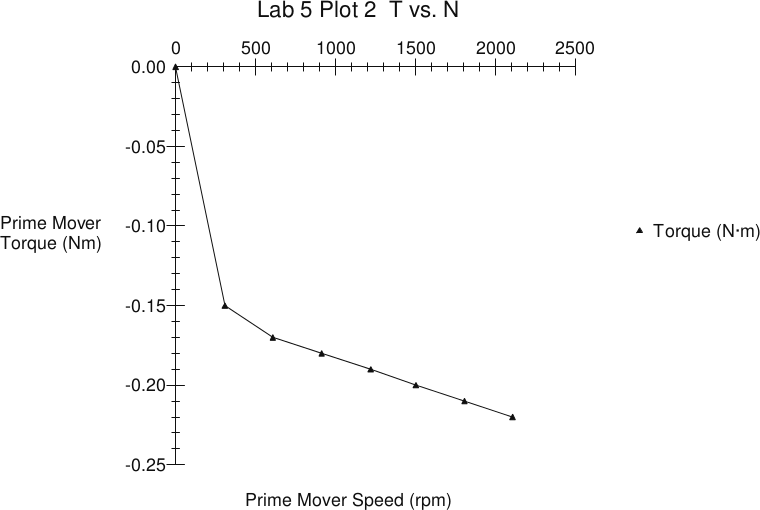
\includegraphics[width=\textwidth]{img/plot2}
  \caption{\gls{pm} friction torque vs. \gls{pm} Speed}
  \label{fig:plot_02}
\end{figure}

\subsection{Dynamometer Operation}

\begin{table}[H]
  \centering
  \begin{tabular}{*{5}{c}}
    $n$ rpm & $T_{DYN}$ N-m& $T_{PM}$ N-m & $T_{NC}$ N-m & $T_C$ N-m \\
    \hline
    1500 &   0 & -0.66 &  --- &  --- \\
    1500 & 2.0 & -2.26 & 1.76 & 2.33 \\
  \end{tabular}
  \caption{\gls{pm} non-corrected and corrected torques}
  \label{tab:table_03}
\end{table}

\subsection{Motor Losses and Efficiency}

\begin{table}[H]
  \centering
  \begin{tabular}{*{2}{c}}
    $T_{C}$ N-m& $N$ rpm \\
    \hline
    1.31 & 1337  \\
  \end{tabular}
  \caption{Dynamometer speed and corrected output torque for a dyno torque of 1.0 Nm}
  \label{tab:table_04}
\end{table}

\begin{table}[H]
  \centering
  \begin{tabular}{*{4}{c}}
    & \textbf{Measured} & \textbf{Calculated} & \textbf{Percent Deviation} \\
    \hline
    $P_{mech}$ N-m & 182.2 & 183.4  & 0.65  \\
    $P_{in}$ N-m & 241.5 & --- & --- \\
    $P_{loss}$ N-m & 59.3 & --- & --- \\
    $\eta$ \% & 75.5 & 75.45 & 0.60 \\
  \end{tabular}
  \caption{Measured and calculated values for mechanical power output,
    electrical power input, and \gls{pm} efficiency; computed \gls{pm}
  power losses}
  \label{tab:table_05}
\end{table}

\begin{table}[H]
  \centering
  \begin{tabular}{*{7}{c}}
    \multicolumn{3}{c}{\textbf{Input}} & \multicolumn{3}{c}{\textbf{Output}}
    & \\

    \textbf{Voltage} & \textbf{Current} & \textbf{Electrical} &
    \textbf{Torque}  & \textbf{Speed}   & \textbf{Mechanical} &
    \textbf{Efficiency} \\

    &                  & \textbf{Power}      &
    &                  & \textbf{Power}
    & \\

    $E_1$ V          & $I_1$ I          & $PQS_1$ W           &
    $T$ N-m          & $N$ rpm          & $P_{m}$ W           &
    $A$ $\eta$ \\

    \hline

    88.71 & 0.94 &  89.90 & 0.32 & 1525.44 &  51.03 & 56.76 \\
    87.42 & 1.25 & 116.22 & 0.48 & 1474.08 &  74.44 & 64.05 \\
    86.08 & 1.58 & 144.32 & 0.67 & 1436.68 & 100.54 & 69.67 \\
    84.88 & 2.02 & 180.53 & 0.90 & 1394.14 & 131.70 & 72.96 \\
    83.98 & 2.40 & 210.73 & 1.11 & 1362.04 & 158.61 & 75.27 \\
    83.21 & 2.77 & 239.24 & 1.31 & 1340.72 & 183.39 & 76.65 \\
    82.42 & 3.13 & 267.18 & 1.50 & 1309.10 & 205.88 & 77.06 \\
    81.67 & 3.53 & 297.42 & 1.71 & 1273.63 & 227.89 & 76.62 \\
    81.01 & 3.90 & 325.22 & 1.92 & 1256.24 & 252.54 & 77.65 \\
    80.34 & 4.24 & 349.83 & 2.08 & 1232.10 & 268.29 & 76.69 \\
    79.57 & 4.64 & 379.02 & 2.30 & 1208.88 & 291.42 & 76.89 \\
  \end{tabular}
  \caption{Recorded values as the Dynamometer's torque was increased}
  \label{tab:table_06}
\end{table}

\begin{figure}[H]
  \centering
  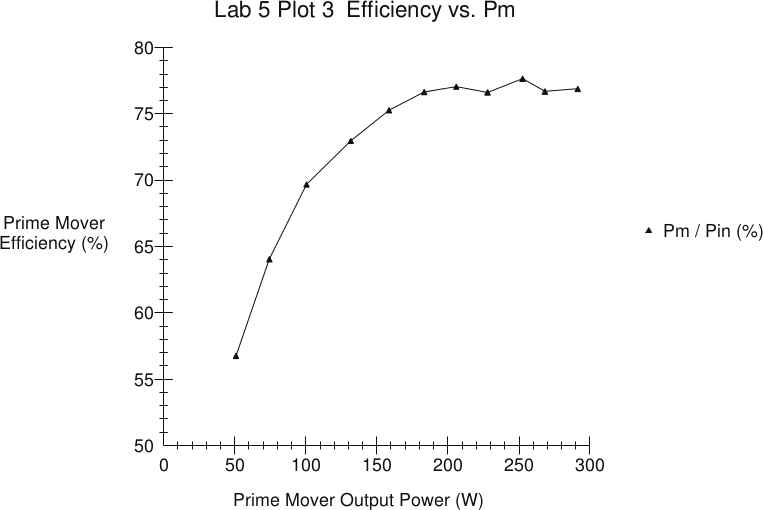
\includegraphics[width=\textwidth]{img/plot3}
  \caption{\gls{pm} efficiency vs.\ mechanical output power}
  \label{fig:plot_03}
\end{figure}

\section{Conclusions}

In Figure~\ref{fig:plot_02}, as the \gls{pm} was first starting to increase
there was a large increase in torque in the opposite direction of motion.
However, as the \gls{pm} gained rotational speed, the opposition torque
continued to increase but at a slower rate. In Figure~\ref{fig:plot_03}, as the
mechanical output power increased, the efficiency also increased. This was
because of the relationship between output power and input power. As the output
power became closer to the value of the input power, then the efficiency of the
motor became closer to 1.

In Part 2, when the \gls{dyno} was connected to the \gls{pm}, the \gls{pm}
generated a larger torque than it generated without the \gls{dyno}. This was
because of the added belt friction and friction torque of the \gls{dyno}
bearings.  When the \gls{dyno} was set to generate its own magnetic torque of
2-Nm, the \gls{pm} rotational speed decreased and thus its opposition torque in
the opposite direction of motion increased. The non-corrected torque generated
by the \gls{pm} was without the loading of the \gls{dyno} taken into account.
When the the corrected torque was generated, the \gls{dyno} loading was taken
into account and thus this value represented the true torque produced by the
\gls{pm}. The corrected torque was greater than the non-corrected torque by
approximately the same amount that the \gls{pm} generated when the \gls{dyno}
had not produced its own magnetic torque.

In Part 3, the current was being increased because the \gls{pm}/\gls{dyno} was
set up as a motor. As the torque produced by the \gls{dyno} increased, the
voltage produced by the \gls{pm} decreased. However, the current increased as
the \gls{pm} rotational speed decreased. The mechanical output power was less
than the electrical input power. Electric power was being converted to
mechanical power.

\section*{Equations}

\[P_{mech}\ = \left( \frac{60}{2\pi} \right) (n \cdot T)\]
\[P_{loss} = P_{in} - P_{mech}\]

\section*{Circuits Tested}

\begin{figure}[H]
  \centering
  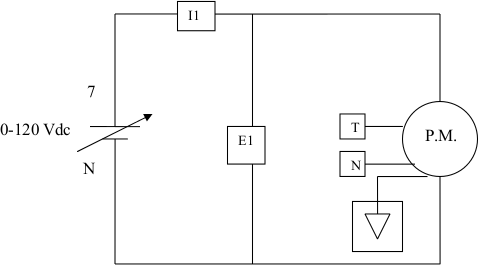
\includegraphics[width=0.8\textwidth]{img/circuit_01}
  \caption{Prime Mover Circuit}
  \label{fig:circuit_01}
\end{figure}

\begin{figure}[H]
  \centering
  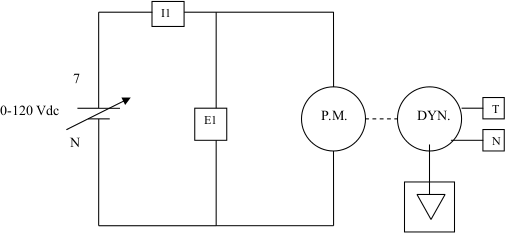
\includegraphics[width=0.8\textwidth]{img/circuit_02}
  \caption{Prime Mover Coupled to the Dynamometer}
  \label{fig:circuit_02}
\end{figure}

\end{document}
